%!TEX root = ../Thesis.tex
%!Mode:: "TeX:UTF-8"

\newcommand*{\ltxcmdname}[1]{\texttt{\textbackslash #1}}
\newcommand*{\ltxenvname}[1]{\texttt{#1}}
\newcommand*{\dif}{\mathop{}\!\mathrm{d}}
\newcommand*{\tc}[1]{\multicolumn{1}{c|}{#1}} %单元格居中对齐

\newcommand*{\figref}[1]{图~\ref{#1}~}
\newcommand*{\secref}[1]{~\ref{#1}~节}
\newcommand*{\tabref}[1]{表~\ref{#1}~}
\newcommand*{\algoref}[1]{算法~\ref{#1}~}
\newcommand*{\codref}[1]{程序~\ref{#1}~}
\newcommand*{\thmref}[1]{定理~\ref{#1}~}
\newcommand*{\axmref}[1]{公理~\ref{#1}~}
\newcommand*{\lemref}[1]{引理~\ref{#1}~}
\newcommand*{\prpref}[1]{命题~\ref{#1}~}
\newcommand*{\defref}[1]{定义~\ref{#1}~}

\newcommand*{\ntcite}[1]{~\cite{#1}~}
\newcommand*{\npcite}[1]{\textsuperscript{\cite{#1}}}

\chapter{智能信息处理实验室毕业论文撰写指南}

\section{对基础模板的调整}

%\subsection{字体}
在基础模板关于英文字体和数学字体的设置中,若发现系统中存在开源的XITS字体(XITS-Regular.otf,一般会包含在几大主流 \LaTeX{} 发行版中),
则会将所有英文字体都设置为XITS,这是一种不好的做法。因为XITS字体作为英文衬线字体(serif font)和数学字体的一种开源替代品,本身只是一种times字体,
原模板强行将英文非衬线字体(sans-serif font)、等宽(mono)或打字机(typewrite)字体
都设置成XITS这种times字体,这显然不符合英文排版基本规则。而且用times字体排版那些需要使用等宽字体的内容(典型的如计算机代码等)既不美观又不利于阅读。
因此,此处建议对其进行调整。最简单的做法是直接停用XITS字体,将artratex.sty文件中的“XITS-Regular.otf”改成“NoXITS-Regular.otf”,
使得 \LaTeX{} 找不到该文件而使相关设置失效。如果不得不用XITS字体,则至少在artratex.sty文件中将设置英文非衬线字体和等宽字体的部分注释掉。

关于中文编码和字体,最新的\LaTeX{} 发行版(例如TeX Live 2020等)的支持已经非常完善,但是建议编译时使用 \XeLaTeX{} (\texttt{xelatex})作为编译引擎,
因为 \XeLaTeX{} 对中文编码、字体及中英文混排的支持要比 pdfLaTeX 强太多。
另外需要注意的一点是,强烈建议在所使用的文本编辑工具中将文字编码设置为UTF-8(在Sublime Text 3和TeXstudio中均为默认编码格式),以免不必要的麻烦。

对于中文字体,基础模版已经预设好了大部分格式排版所对应的中文字体,例如章节标题为黑体、正文为宋体,配合英文的\textbf{加粗Text}使用宋体伪粗体、
\textit{斜体Text}使用楷体、\texttt{等宽Text}使用仿宋体等。基础模板使用“伪粗体(\texttt{AutoFakeBold})”的方式定义中文宋体和黑体的粗体字型,
这种方式本质上就是将文字横向以微小位移重复显示多次而呈现出加粗效果,即使在计算机中文字体设计很不规范、缺少对应变化字型的年代,
这也是一种不被推荐的折衷方案,不仅效果差强人意,而且会对生成的pdf文件中的文字拷贝造成困扰。
因此,建议使用比较新的中文开源字体:由Adobe和Google联合开发的\href{https://github.com/adobe-fonts}{思源字体}
(加载文档类\texttt{ucasthesis}时加上参数“\texttt{fontset=none}”)。即使不使用这种方式,也应修改字体配置,去掉\texttt{AutoFakeBold}选项,
而代之以其他替代字体(例如用Microsoft Office软件一般都会捆绑安装的“华文中宋”字体作为宋体的粗体)。

另外,修改后的模版为“\texttt{fontset=none}”选项补充定义了4种常用中文字体,方便撰写正文时快速切换字体,
分别是:{\songti 宋体}、{\heiti 黑体}、{\kaishu 楷书}、{\fangsong 仿宋}。

关于在 \LaTeX{} 中使用中英文字体的基础常识及相关设置方法可参考:\href{https://stone-zeng.github.io/2018-08-08-use-opentype-fonts/}{在 \LaTeX{} 中使用 OpenType 字体}。

\section{撰写样例}\label{sec:samples}

\subsection{列表}
\LaTeX{} 用于列表的环境有三种:\texttt{itemize}、\texttt{enumerate}和\texttt{description}。

无序列举:
\begin{itemize}
	\item 列举项
	\item 列举项
\end{itemize}

带序号列举:
\begin{enumerate}
	\item 列举项
	\item 列举项
\end{enumerate}

带序号列举可以设定序号格式:
\begin{enumerate}[1).]
	\item 列举项
	\item 列举项
\end{enumerate}

带标签的列举,适用于名词定义:
\begin{description}
	\item[名词1] 解释1
	\item[Name2] Description2
\end{description}

列表环境可以相互嵌套,起始编号可以用 \ltxcmdname{setcounter} 命令改变:
\begin{enumerate}
    %用\setcounter改变起始编号,注意:counter从0起计数,显示的序号为当前counter的值加1
    %所以要设置序号从n开始的话,调用\setcounter{enumi}{n-1}
    \setcounter{enumi}{3}
	\item 列举项
    \begin{itemize}
    	\item 列举项
    	\item 列举项
    \end{itemize}
	\item 列举项
	\begin{enumerate}
    	\item 列举项
    	\item 列举项
	\end{enumerate}
\end{enumerate}


\subsection{数学公式}
段落内的数学公式,有三种输入方式:$E=mc^2$、\(\frac{1}{2}\sqrt{b^2-4ac}\)、\begin{math}\mathbf{n}=[x, y, z]^T\end{math}。

段落间的数学公式也有对应的三种输入方式:
% (1)
$$A=\int_0^1 \frac{\ln{x}}{x}\dif x$$
% (2)
\[
A=\int_0^1 \frac{\ln{x}}{x}\dif x
\]
% (3)
\begin{displaymath}
A=\int_0^1 \frac{\ln{x}}{x}\dif x
\end{displaymath}

带编号的数学公式:
\begin{equation}\label{eq:samples:one}
A=\int_0^1 \frac{\ln{x}}{x}\dif x
\end{equation}

带编号的数学公式组(注意利用列分隔符“\texttt{\&}”对齐):
\begin{align}
\mathcal{M}^2(\hat{\theta},\theta) &= E[(\hat{\theta} - \theta)^2] \\
\mathcal{M}^2(\hat{\theta},\theta) &= \operatorname{var}^2(\hat{\theta}) + {\cal B}^2(\hat{\theta})
\end{align}

\textbf{特别注意:}此处应避免使用 \ltxenvname{eqnarray} 环境,因为此环境存在很多问题,且与\ltxenvname{amsmath}宏包风格不统一,
具体问题请参考这篇文章“\href{https://tug.org/pracjourn/2006-4/madsen/madsen.pdf}{Avoid eqnarray!}”。

跨行长公式(注意利用“\texttt{\&}”对齐):
\begin{equation}
\begin{split}
a& =b+c-d\\
 & \quad +e-f\\
 & =g+h\\
 & =i
\end{split}
\end{equation}

带子编号的数学公式组:
\begin{subequations}\label{eq:samples:grp}
\begin{align}
a&=b+c\label{eq:samples:grp:a}\\
d&=e+f+g\label{eq:samples:grp:b}\\
h&=i+j\label{eq:samples:grp:c}
\end{align}
\end{subequations}

大型分式:
\begin{equation}
\Re{z} =\frac{n\pi \dfrac{\theta +\psi}{2}}{
        \left(\dfrac{\theta +\psi}{2}\right)^2 + \left( \dfrac{1}{2}
        \log \left\lvert\dfrac{B}{A}\right\rvert\right)^2}.
\end{equation}

带条件赋值:
\begin{equation}
z = \left\{
\begin{array}{ll}
1 & (x>0)\\
0 & (x<0)
\end{array}
\right.
\end{equation}

矩阵的输入用 \texttt{matrix} 环境,以“\texttt{\&}”分列、以“\ltxcmdname{\textbackslash}”或“\ltxcmdname{cr}”分行,下面是一个例子:
\begin{equation}
\left(
  \begin{matrix}
    K_{11} &K_{12} &K_{13} &\ldots &K_{1n}\\
    K_{21} &K_{22} &K_{23} &\ldots &K_{2n}\\
    K_{31} &K_{32} &K_{33} &\ldots &K_{3n}\\
    \vdots &\vdots &\vdots &\ddots &\vdots\\
    K_{n1} &K_{n2} &K_{n3} &\ldots &K_{nn}
  \end{matrix}
\right) \left(
  \begin{matrix}
     D_{1}\\ D_{2}\\ D_{3}\\ \vdots\\ D_{n}
  \end{matrix}
\right) = \left(
  \begin{matrix}
    F_{1}\\ F_{2}\\ F_{3}\\ \vdots\\ F_{n}
  \end{matrix}
\right)
\end{equation}

正文中对公式的引用一律使用\ltxcmdname{eqref}命令输出带括号的公式编号,例如:公式~\eqref{eq:samples:one}。

关于数学公式的特别提示:
\begin{enumerate}
  \item \textbf{多字母的函数或算子名称表示要规范}:多字母的函数或算子名称在~\LaTeX{}中有专门的排版方式,一些常用的已经定义了专门的命令,
        例如\ltxcmdname{sin}、\ltxcmdname{max}、\ltxcmdname{log}等,对于一些\ltxenvname{amsmath}包中未定义的函数,一定要在数学环境中用\ltxcmdname{operatorname}命令括起来,
        例如:\ltxcmdname{operatorname\{softmax\}(A)}就显示为$\operatorname{softmax}(A)$,这和在数学环境中用\ltxcmdname{text}(显示为$\text{softmax}(A)$)或
        直接写(显示为$softmax(A)$)都有差别,后者尤为错误。
  \item \textbf{尽量不要使用多字母变量}:在数学环境中直接输出多字母变量会产生歧义,数学环境中默认的排版规则认为每一个英文字母都是一个单独的变量,在字符间距的处理上有特殊的考虑,
        若直接输入多字母变量,则各个字母间会分得比较开,例如:$Ver_i$,读者容易看成$V$、$e$和$r_i$的乘积,因此数学公式中要避免使用多字母变量。
        在这里,一条重要的原则是:数学公式要经过一定的提炼和抽象,不要直接从程序代码翻译,即不要在数学公式的表达中带入写程序的习惯。\label{enum:mathtips:1}
  \item \textbf{不同类型的数学符号尽量用不同的字体表示}:不同类型的数学符号用不同类型的字体表示有利于增加公式的辨识度,使读者更易理解,例如矩阵和向量一般用粗体,
        $\mathbf{Ax}=\mathbf{b}$就比$Ax=b$含义更明确。
  \item \textbf{用有意义的单词做变量上下标时单词要放在文本环境中}:有时候为了表达更简洁明了,会在变量的上标或下标用单词表示某些特殊含义,例如$A_\text{max}$,
        此时,用来表达特殊含义的单词务必放在\ltxcmdname{text}命令中,理由同~\ref{enum:mathtips:1}。
\end{enumerate}

\subsection{插图}
为了能得到较好的排版效果,又不必做调整图形位置的乏味工作,\LaTeX{} 提供了一个浮动图形机制来自动将图形放置到合适的位置。为了使这一机制发挥最大效力,在写作时需注意以下几点:
\begin{enumerate}
	\item \textbf{不要使用依赖于图形放置位置的文本}:使用如“\emph{这幅图…}”或“\emph{下图…}”等短语要求所指图形需在固定位置,
	      而像“{\kaishu 图1-1…}”这样的短语则允许图形出现在任意位置,而且配合\LaTeX{} 提供的强大的交叉引用功能,
	      完全可以自动生成插图编号并建立超链接。
	\item \textbf{放轻松}:一些刚开始使用\LaTeX{} 的作者发现图形没有十分准确地出现在他们所想要的位置,往往会着急,并对其进行手工干预,
	      这其实完全没有必要,图形的放置是\LaTeX{} 的工作,最好放轻松一些,等所有内容都撰写校对完成,最后再对插图位置作必要微调。
	      如果你的论文结构合理,正文内容完整充实,此时你会发现插图都已在该在的位置上,没有调整的必要了。
\end{enumerate}

插图一般被放置在\ltxenvname{figure}环境中,\figref{fig:samples:coordinateaxis}是一个单幅插图的例子。\ltxenvname{figure}环境有一个可选参数允许用户指示图形有可能被放置的位置(实际上所有浮动对象环境均有类似的参数设置,例如\secref{sec:tab}要讲的表格环境),这一选项参数可以是下列字母的任意组合(缺省为\texttt{[tbp]}):
\begin{description}
	\item[\texttt{h}(当前位置)] 将插图放置在正文文本中figure环境出现的地方,如果当前页所剩空间不够,这一参数将不起作用;
	\item[\texttt{t}(顶部)] 将插图放置在页面顶部;
	\item[\texttt{b}(底部)] 将插图放置在页面底部;
	\item[\texttt{p}(浮动页)] 将插图放置在只允许有浮动对象的页面上
\end{description}

通常给出的参数越多,\LaTeX{} 的排版效果越好,例如\texttt{[htbp]}、\texttt{[tbp]}、\texttt{[htp]}、\texttt{[tp]}等组合的效果都不错。另外,在这些位置参数前面加上一个惊叹号(例如\texttt{[!ht]})会使\LaTeX{} 忽略应用于文本页的审美条件,试图用最严格的标准来放置浮动图形。

\figref{fig:samples:coordinateaxis}是单幅插图的例子。

%% 单幅插图
\begin{figure}[htbp]
%%图形居中放置
\centering
%%插入图形文件
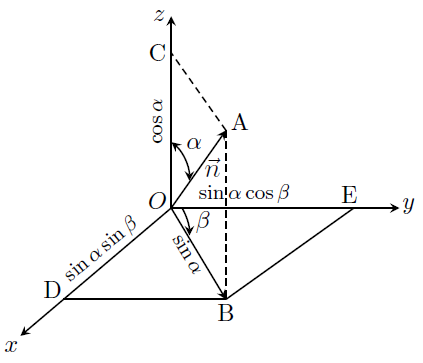
\includegraphics[width=0.45\textwidth]{coordinateaxis}
%                         ^                 ^
%                插图宽度(相对于文本宽)  插图文件名(忽略扩展名)
%% 插图标题(\label 用于设置建立交叉引用的标签名)
\bicaption{平面的倾角、倾向及其法向矢量}{Dip, dip direction and normal vector of a plane}\label{fig:samples:coordinateaxis}
\end{figure}

\figref{fig:samples:blcfy}是包含子图的例子,在\texttt{figure}环境中嵌套\texttt{subfigure}环境即可,参数格式类似,唯一不同的是\texttt{subfigure}不是一个浮动对象(被限制在\texttt{figure}中),因此其位置参数是指子图对齐的方式:\texttt{b}表示底部对齐,\texttt{t}表示顶部对齐。子图间可以用“\ltxcmdname{\textbackslash}”换行。

%% 包含子图的插图
\begin{figure}[htbp]
\def\figwidth{\columnwidth}
  \centering
    \begin{subfigure}[b]{0.5\figwidth} %子图宽度(用相对于整个figure的比例指定)
      \centering
      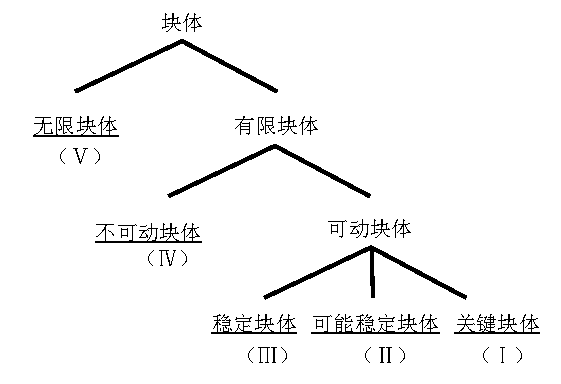
\includegraphics[width=\textwidth]{blockclassify}
      \caption{块体类型}\label{fig:samples:blockclassify}
    \end{subfigure} %此处可以用“\\”换行
    \begin{subfigure}[b]{0.36\figwidth}
      \centering
      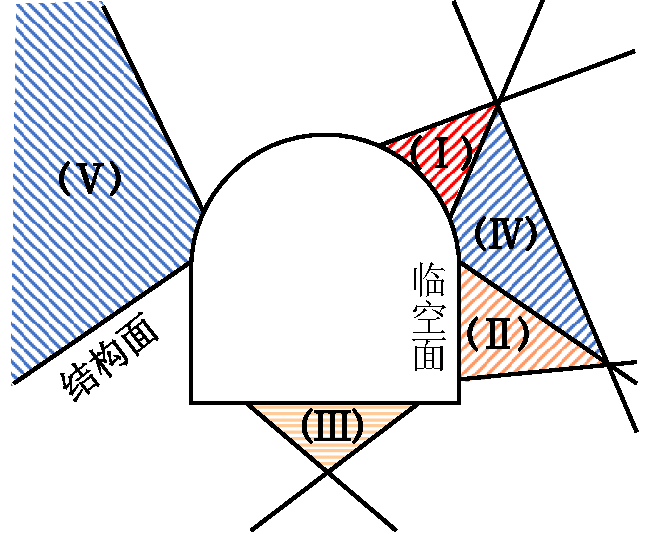
\includegraphics[width=\textwidth]{blockclassify1}
      \caption{平面示意图}\label{fig:samples:blockclassify1}
    \end{subfigure}
  \bicaption{块体分类}{Block classification}\label{fig:samples:blcfy}
\end{figure}

特别注意,模版支持多种常用插图文件格式,比如\texttt{pdf}、\texttt{png}、\texttt{jpg}、\texttt{tif}等,在用\ltxcmdname{includegraphics}命令引入插图文件时,文件名可以不包含扩展名,\LaTeX{} 会自行匹配,这样做的好处是当你用另一种更好的文件格式提供同一幅插图时(比如用效果更好的矢量图格式\texttt{pdf}代替原来不够清晰的\texttt{jpg}文件),直接替换插图文件即可,正文中不需要做任何更改。

另外,关于图表的标题,由于学校毕业论文模板要求同时给出中、英文标题,因此在排版图表标题时使用“\ltxcmdname{bicaption}”,其格式为:
\begin{verbatim}
  \bicaption[中文短标题]{中文标题}
            [Short English title]{Title in English}
\end{verbatim}
其中,方括号中的可选参数为出现在目录等其他文档结构中的标题,当图表标题很长或者包含一些不宜出现在目录中的额外标记(如文献引用标注等)时,可使用该可选参数调整呈现在目录中的标题。

\subsection{表格}\label{sec:tab}
表格和插图一样,建议使用浮动对象,即将表格放在浮动对象环境\texttt{table}中,例如\tabref{tab:samples:normal}。但是也有一些例外,例如跨页的长表格\texttt{longtable}(\tabref{tab:samples:longtable}),由于不受页面长度限制,所以不必放在浮动对象中,放进去反而会出错。

%% 普通表格
\begin{table}[htbp]
\bicaption{普通表格示例}{Sample for the normal table}\label{tab:samples:normal}
\centering
\begin{tabular}{|>{\tt}c|>{\kaishu}l|>{\tt}l|>{\kaishu}l|}
\hline
  \heiti 变量名 & \tc{\heiti 含义}    & \tc{\heiti 类型} & \tc{\heiti 备注} \\ \hline
  id           & 唯一标识符           & int             & 必须有            \\ \hline
  name         & 名称                & string          &                  \\ \hline
  abbrName     & 名称简写             & string          &                  \\
\hline
\end{tabular}
\end{table}

表格内容的输入则要比插图复杂一些,一般放在\texttt{tabular}环境中,也有的直接放在对应表格环境中(如\texttt{longtable}),列选项在表格环境参数中设置,不同的表格环境其内容大同小异。表格正文内容则一致以“\texttt{\&}”分列、以“\ltxcmdname{\textbackslash}”或“\ltxcmdname{tabularnewline}”换行。表格环境列布局的参数设置比较灵活,可以设定每一列的对齐方式(\texttt{l}、\texttt{r}或\texttt{c},有几个就有几列)、字体(放在“\texttt{>}”后的大括号内)、是否加列间线(“\texttt{|}”)等(详细说明可参考\tabref{tab:samples:longtable})。

此外,还可以使用 \ltxcmdname{multirow}、\ltxcmdname{multicolumn}等命令合并单元格,例如\tabref{tab:samples:threepart}。
\begin{enumerate}
	\item 多行单元格:\ltxcmdname{multirow\{nrows\}[bigstructs]\{width\}[fixup]\{text\}}。其中:\texttt{nrows}设定所占用的行数;\texttt{bigstructs}为可选项,主要是在使用了 bigstruct 宏包时使用;\texttt{width}设定该栏文本的宽度,如果想让 LaTeX 自行决定文本的宽度,则用 * 即可;\texttt{fixup}为可选项,主要用来调整文本的垂直位置;\texttt{text}为所要排版的文本,可用“\ltxcmdname{\textbackslash}”来强制换行。
    \item 多列单元格:\ltxcmdname{multicolumn\{ncols\}\{align\}\{text\}}。其中:\texttt{ncols}设定所占用的列数;\texttt{align}是列选项参数,类似于\texttt{tabular}环境参数,如“\texttt{|c|}”;\texttt{text}为所要排版的文本。
\end{enumerate}

此外,\tabref{tab:samples:threepart}也使用了一个特殊的表格环境\texttt{threeparttable}来生成三线表,此环境主要用处是提供了在表格内加脚注的功能,同时也预定义了一些画各种粗细线条的命令,用于生成不同粗细的表格横线。

%% 三线表及不规则单元格示例
%   (1) 跨行混排
%       \multirow{nrows}[bigstructs]{width}[fixup]{text}
%        nrows       设定所占用的行数。
%        bigstructs  此为可选项,主要是在你使用了 bigstruct 宏包时使用。
%        width       设定该栏文本的宽度。如果想让 LaTeX 自行决定文本的宽度,则用 * 即可。
%        fixup       此为可选项,主要用来调整文本的垂直位置。
%        text        所要排版的文本。可用 \\ 来强迫换行。
%   (2) 跨列混排
%       \multicolumn{ncols}{align}{text}
%        ncols  设定所占用的列数。
%        align  列选项参数,类似于tabular环境参数,如“|c|”。
%        text   所要排版的文本。
\begin{table}[htbp]
\centering
  \begin{threeparttable}
    \newcommand{\chengs}{\ensuremath{\times}}
    \newcommand{\cheng}{\ensuremath{\!\times\!}}
    \bicaption{三线表及不规则单元格示例}{Sample for the three-line table and irregular cells}\label{tab:samples:threepart}
    \begin{tabular}{cccc} %指定列数以及每列文字对齐方式:l 左对齐、r 右对齐、c 居中
      \toprule
  \multirow{2}{*}{策略}   & \multirow{2}{*}{尺寸参数}             & \multicolumn{2}{c}{数据量}    \tabularnewline \cmidrule{3-4}
                         &                                      & 数据块数\tnote{a} & 读取像素数\tnote{b} \tabularnewline \midrule
  \multirow{2}{*}{等分}   & $48\chengs 48\chengs 48$             & 2058             & 227598336 \tabularnewline \cmidrule{2-4} %从第2列到第4列画横线
                         & $128\chengs 128\chengs 128$          & 155              & 325058560 \tabularnewline \midrule
  \multirow{2}{*}{自适应} & $[16,64]\cheng[16,64]\cheng[16,64]$  & 1100             & 211624837  \tabularnewline \cmidrule{2-4}
                         & $[16,250]\cheng[16,64]\cheng[16,32]$ & 748              & 219153002  \tabularnewline %“\tabularnewline”相当于“\\”
      \bottomrule
    \end{tabular}
    \begin{tablenotes}\small
      \item[a] 每块数据包括边界
      \item[b] 第二个脚注
    \end{tablenotes}
  \end{threeparttable}
\end{table}

\texttt{longtable}环境用于排版跨页长表,与普通表格不太一样,不能当做浮动对象,当它附近有较多浮动表格对象时有可能导致表格出现的顺序和生成的编号顺序不一致,因此如无必要,建议尽量少用跨页长表,对于过长的表格应当进行适当的拆分。

%% 跨页长表
\begin{longtable}{|>{\tt}c|>{\kaishu}m{10cm}|}
  \bicaption[跨页长表示例]{跨页长表示例及表格列选项参数说明}{Sample for the long table over multiple pages and description for the parameters} \label{tab:samples:longtable}\\
    \hline \heiti 选项参数 & \tc{\heiti 说明} \\ \endfirsthead %第一页上的表头
  %% 出现在续页上的标题有两种排版方法(建议使用bicaption排版):
  % (1) 续页表格的标题、页码不出现在表格目录中,标题和表格纵向间距较小(可自行调整),注意用“\thetable”输出表格编号
  %\multicolumn{2}{c}{\bfseries\small \tablename\ \thetable\ {跨页长表示例及表格列选项参数说明(续表)}} \\
  %\multicolumn{2}{c}{\bfseries\small Table\ \thetable\ {Sample for the long table over multiple pages and description for the parameters (continued)}} \\
  % (2) 使用常规caption或bicaption排版,标题、页码将出现在表格目录中
  %\caption[跨页长表示例(续表)]{跨页长表示例及表格列选项参数说明(续表)} \\
  \bicaption[跨页长表示例(续表)]{跨页长表示例及表格列选项参数说明(续表)}{Sample for the long table over multiple pages and description for the parameters (continued)} \\
    \hline \heiti 选项参数 & \tc{\heiti 说明} \\ \endhead %出现在续页上的表头
    \hline         l      & 该列单元格内容左对齐 \\
    \hline         c      & 该列单元格内容居中 \\
    \hline         r      & 该列单元格内容右对齐 \\
    \hline     p\{width\} & 将内容放进一个宽为\texttt{width}的段落盒,等价于\ltxcmdname{parbox[t]\{width\}} \\
    \hline     @\{decl.\} & 删除两边列之间的空白,插入指定的文本,即大括号间的内容\texttt{decl.} \\
    \hline     m\{width\} & 指定列宽为\texttt{width},超出宽度的文字将自动换行,作用接近\ltxcmdname{parbox\{width\}} \\
    \hline     b\{width\} & 相当于\ltxcmdname{parbox[b]\{width\}} \\
    \hline     >\{decl.\} & 可在每个列选项字母之前使用,将大括号间的内容(\texttt{decl.})插入到该列每个单元格内容之前,可以用它来控制每一列的文本格式 \\
    \hline     <\{decl.\} & 可在每个列选项字母之后使用,将大括号间的内容(\texttt{decl.})插入到该列每个单元格内容之后,配合“\texttt{>}”使用可方便地将该列每个单元格放置在一个环境中,比如数学环境 \\
    \hline          |     & 插入一条竖线 \\
    \hline     !\{decl.\} & 与\texttt{|}类似,只不过插入的不是竖线而是大括号间的内容(\texttt{decl.})  \\
    \hline
\end{longtable}

对于较宽的表格,可以使用“\ltxenvname{landscape}”环境按横排方式进行排版,如\tabref{tab:samples:landscapelongtable}所示,此表格也演示了在横排环境下的跨页长表排版。
此外,跨页表格的标题与一般表格有所不同,需额外提供续表标题,排版格式如下:
{\linespread{1.2}
\begin{verbatim}
  \bicaption[短标题]{标题}[Short title]{Title} \label{...} \\
    \hline 列名1 & 列名2 & ... \\ \endfirsthead %第一页上的表头
  \bicaption[短标题(续表)]{标题(续表)}
            [Short title (continued)]{Title (continued)} \\
    \hline 列名1 & 列名2 & ... \\ \endhead %出现在续页上的表头
\end{verbatim}}

\begin{landscape}% 横排页环境
\pagestyle{lscape}% 横排页眉页脚样式
\begin{longtable}{|>{\tt}c|>{\kaishu}m{10cm}|}
  \bicaption[横排跨页长表示例]{横排跨页长表示例及表格列选项参数说明}{Sample for the landscape-oriented long table over multiple pages and description for the parameters} \label{tab:samples:landscapelongtable}\\
    \hline \heiti 选项参数 & \tc{\heiti 说明} \\ \endfirsthead %第一页上的表头
  %\multicolumn{2}{c}{\bfseries\small \tablename\ \thetable\ {横排跨页长表示例及表格列选项参数说明(续表)}} \\
  %\multicolumn{2}{c}{\bfseries\small \tablename\ \thetable\ {Sample for the landscape-oriented long table over multiple pages and description for the parameters (continued)}} \\
  %\caption[横排跨页长表示例]{横排跨页长表示例及表格列选项参数说明(续表)} \\
  \bicaption[横排跨页长表示例(续表)]{横排跨页长表示例及表格列选项参数说明(续表)}{Sample for the landscape-oriented long table over multiple pages and description for the parameters (continued)} \\
    \hline \heiti 选项参数 & \tc{\heiti 说明} \\ \endhead %出现在续页上的表头
    %\hline \multicolumn{2}{r}{\textit{续表见下页}}\\ \endfoot %续表脚注
    %\endlastfoot %最后一页脚注
    \hline         l      & 该列单元格内容左对齐 \\
    \hline         c      & 该列单元格内容居中 \\
    \hline         r      & 该列单元格内容右对齐 \\
    \hline     p\{width\} & 将内容放进一个宽为\texttt{width}的段落盒,等价于\ltxcmdname{parbox[t]\{width\}} \\
    \hline     @\{decl.\} & 删除两边列之间的空白,插入指定的文本,即大括号间的内容\texttt{decl.} \\
    \hline     m\{width\} & 指定列宽为\texttt{width},超出宽度的文字将自动换行,作用接近\ltxcmdname{parbox\{width\}} \\
    \hline     b\{width\} & 相当于\ltxcmdname{parbox[b]\{width\}} \\
    \hline     >\{decl.\} & 可在每个列选项字母之前使用,将大括号间的内容(\texttt{decl.})插入到该列每个单元格内容之前,可以用它来控制每一列的文本格式 \\
    \hline     <\{decl.\} & 可在每个列选项字母之后使用,将大括号间的内容(\texttt{decl.})插入到该列每个单元格内容之后,配合“\texttt{>}”使用可方便地将该列每个单元格放置在一个环境中,比如数学环境 \\
    \hline          |     & 插入一条竖线 \\
    \hline     !\{decl.\} & 与\texttt{|}类似,只不过插入的不是竖线而是大括号间的内容(\texttt{decl.})  \\
    \hline
\end{longtable}
\end{landscape}

\subsection{计算机程序}
计算机源程序可以用 \texttt{lstlisting} 环境排版,代码可直接拷贝进去,除语法高亮外基本原样输出。下面是一个简单的例子:
\begin{lstlisting}
  int PacketQueue::put(AVPacket *pkt) {
      int ret;    
      this->mutex->lock();
      ret = put_private(pkt);
      this->mutex->unlock();    
      if (pkt != &this->flush_pkt && ret < 0) av_packet_unref(pkt);    
      return ret;
  }
\end{lstlisting}

本模版预设按C++语法进行排版及关键字高亮显示,可以用环境参数中切换语言并作其他更细致的设定,例如 \texttt{[language=Pascal]} 将当前 \texttt{lstlisting} 环境切换为 Pascal 语言。同时,页可以通过参数设置将其变为浮动对象:\texttt{[float, caption=A floating example]},如 \codref{lst:samples:pas} 所示。更详细的用法可参考 \texttt{listings} 宏包的说明文档(\texttt{listings.pdf})。
\begin{lstlisting}[float, language=Pascal, caption={浮动代码块}, label={lst:samples:pas}]
  var i:integer;
  var x:integer;
  for i:=maxint to 0 do
  begin
    if (i<=0) then x := 1;
    if (i>0) then x := 0;
  end;
\end{lstlisting}

\subsection{定理}
定理,包括命题、引理、推论等的排版使用 \texttt{theorem}、\texttt{lemma}、\texttt{proposition} 等环境,每个定理可用可选参数指定一个别名。定理的证明放在 \texttt{proof} 环境中,证明结束标志为 \ltxcmdname{qedhere}。

定理示例:
\begin{theorem}[有限性定理] \label{thm:samples:t}
块体为有限的充分必要条件是节理锥(JP)与开挖锥(EP)的交集为空集。
\end{theorem}

公理示例:
\begin{axiom} \label{thm:samples:a}
平面上两点确定一条直线。
\end{axiom}

引理示例:
\begin{lemma} \label{thm:samples:l}
块体为有限的充分必要条件是节理锥(JP)与开挖锥(EP)的交集为空集。
\end{lemma}

命题及证明示例:
\newcommand{\sNP}{\ensuremath{\mathcal{NP}}}
\newcommand{\tNP}{\sNP\ }
\newcommand{\tNPC}{\mbox{\ensuremath{\mathcal{NP}\text{-完全}}}}
\begin{proposition} \label{thm:samples:p}
若有向图的哈密尔顿环路问题是~\tNPC 问题,则无向图的哈密尔顿环路问题也是~\tNPC 问题。
\end{proposition}

\begin{proof}
    显然,无向哈密尔顿环路问题属于~\tNP 问题,因此只要证明有向图的哈密尔顿环路问题可多项式规约到无向图的
    哈密尔顿环路问题~(已知有向图的哈密尔顿问题是~\tNPC 问题)。

    令~$G=(V,E)$ 是包含~$n$ 个顶点的有向图,现将其转换到无向图~$G'=(V',E')$:对每个~$v\in V$,
    $V'$ 中包含~$3$ 个顶点~$v^1,v^2,v^3$ 与之对应,$E'$ 中包含两条无向边~$v^1v^2,v^2v^3$ 与之对应,
    对~$E$ 中的每条边~$vw$,$E'$ 中包含无向边~$v^3w^1$ 与之对应,显然,该转换所需时间以多项式为界,
    若~$|V|=n,|E|=m$ 则~$|V'|=3n,|E'|=2n+m$。

    若~$G$ 中有一条有向哈密尔顿环路~$v_1,\cdots,v_n$,则~$v_1^1,v_1^2,v_1^3,v_2^1,v_2^2,v_2^3,\cdots,$ $v_n^1,v_n^2,v_n^3$ 是~$G'$ 中
    的一条~(无向) 哈密尔顿环路;另一方面,若~$G'$ 中存在一条哈密尔顿环路,由于对每组顶点~$v^1,v^2,v^3$,$v^2$ 只与~$v^1$ 和~$v^3$ 相连,
    因此在环路上必按~$v^1,v^2,v^3$ 或~$v^3,v^2,v^1$ 的顺序访问这三个顶点,而~$G'$ 中的其他边仅连接上标为~$1$ 和~$3$ 的顶点,
    因此该环路上所有的三顶点组要么都按~$1,2,3$ 的顺序排列,要么都按~$3,2,1$ 的顺序排列,
    不妨设该环路为~$v_{i_1}^1,v_{i_1}^2,v_{i_1}^3,\cdots,v_{i_n}^1,v_{i_n}^2,v_{i_n}^3$,则~$v_{i_1},\cdots,v_{i_n}$ 是~$G$ 中的一条
    有向哈密尔顿环路。所以~$G$ 包含有向哈密尔顿环路当且仅当~$G'$ 包含无向哈密尔顿环路。\qedhere
\end{proof}

定义示例:
\begin{definition}[复流形] \label{thm:samples:d}
复流形$M$是一个可微流形,它容许一个开覆盖$\{U_{\alpha}\}$和坐标映射$\varphi_{\alpha}:U_{\alpha}\rightarrow \mathbb{C}^n$ 使得对所有的$\alpha, \beta, \varphi_{\alpha}\circ \varphi_{\beta}^{-1}$在$\varphi_{\beta}(U_{\alpha}\cap U_{\beta})\subset \mathbb{C}^n$是全纯的。
\end{definition}

\subsection{交叉引用}
理论上在文档的任何位置都可以设置交叉引用点,常用的有:特定章节、图、表、公式等。为被引用对象建立交叉引用点的方法是在相应位置使用 \ltxcmdname{label}命令设置一个标签,在需要引用的地方用 \ltxcmdname{ref} 命令建立引用链接,其参数就是前面所设置的标签名称。例如:参见 \ref{sec:samples} 节。由于引用链接只输出\LaTeX{} 为标签自动生成的编号,所以一般要在 \ltxcmdname{ref} 命令的前后配上相应文字,如“图”、“表”、“公式”等。为省去此琐碎环节,本模版预定义了一些固定的引用模式供大家使用,如:章节引用\secref{sec:samples}、插图引用\figref{fig:samples:blcfy}、表格引用\tabref{tab:samples:normal}、算法引用\algoref{alg:euclid}、代码引用\codref{lst:samples:pas}、定理引用\thmref{thm:samples:t}、公理引用\axmref{thm:samples:a}、引理引用\lemref{thm:samples:l}、命题引用\prpref{thm:samples:p}、定义引用\defref{thm:samples:d}等。

另外,还可以使用 \ltxcmdname{pageref}引用对象所在页码,例如:\figref{fig:samples:blcfy}在第 \pageref{fig:samples:blcfy} 页。

页面内的脚注用 \ltxcmdname{footnote}命令添加,例如:此处\footnote{脚注内容。}有脚注。

\subsection{参考文献引用}\label{sec:samples:cite}
模板提供了一组源自\texttt{natbib}包的引用命令用于不同风格的引用习惯:
\begin{center}
%\linespread{0.5}
%\renewcommand{\arraystretch}{1.0}
\begin{tabular}{lcl}
\verb|\citet{wikibook2014latex}| & $\Rightarrow$ & \citet{wikibook2014latex} \\
\verb|\citet[第2章]{wikibook2014latex}| & $\Rightarrow$ & \citet[第2章]{wikibook2014latex} \\
\verb|\citep{wikibook2014latex}| & $\Rightarrow$ & \citep{wikibook2014latex} \\
\verb|\citep[第2章]{wikibook2014latex}| & $\Rightarrow$ & \citep[第2章]{wikibook2014latex} \\
\verb|\citep[见][第2章]{wikibook2014latex}| & $\Rightarrow$ & \citep[见][第2章]{wikibook2014latex}
\end{tabular}
\end{center}

其中,后缀“\texttt{t}”表示“textual”,即句中(文本中的)引用,也就是引用本身是句子的一个成分;
后缀“\texttt{p}”表示“parenthetical”,即句末(括号里的)引用,作为一个插入语(附加说明)存在。请自行体会其中的区别。

但以上命令主要为英文文献设计,有些地方并不是很符合中文的习惯。在中文文献中,若使用数字序号形式的引用标注,
句末引用一般采用上标形式,句中引用则仍使用正常形式。但在基础模板中,虽然提供了“\texttt{super}”文档参数支持上标形式的引用标注,
但却是一股脑把所有标注命令全改成的上标形式,不是很合理。因此,若采用数字序号形式的引用标注,必要时可直接用“\ltxcmdname{cite}”命令自行排版。

为便于后期统一修改引用标注风格,建议根据自己的需要自行定义相关命令,简化论文撰写过程,例如在“\texttt{Thesis.tex}”文件的导言区或“\texttt{artracom.sty}”
加入相关自定义命令:{\linespread{1.1}
\begin{verbatim}
  \newcommand*{\ntcite}[1]{~\cite{#1}~}
  \newcommand*{\npcite}[1]{\textsuperscript{\cite{#1}}}
\end{verbatim}}
用于生成不同位置的文献引用标注,此处文献\ntcite{wikibook2014latex}是句中引用(文献本身是句子成分之一),这是句末(上标,文献不是句子成分之一,仅表示名词或句子来自哪篇文献)引用\npcite{wikibook2014latex}。

参考文献信息记录在“\texttt{.bib}”文件中,务必保证每一条文献信息完整、准确,建议用开源软件~\href{https://www.jabref.org/}{JabRef}~进行信息录入和管理。
